\documentclass{standalone}
\usepackage{tikz}
\usepackage{amsmath}
\usetikzlibrary{calc, tikzmark, shapes, shapes.arrows, arrows, positioning}
\usetikzlibrary{decorations.fractals,%
decorations.shapes,%
decorations.text,%
decorations.pathmorphing,%
decorations.pathreplacing,%
decorations.footprints,%
decorations.markings}

\newcommand{\mat}[1]{\boldsymbol{\mathrm{#1}}}
\newcommand{\avg}[1]{\left\{\!\!\left\{#1\right\}\!\!\right\}}

\begin{document}
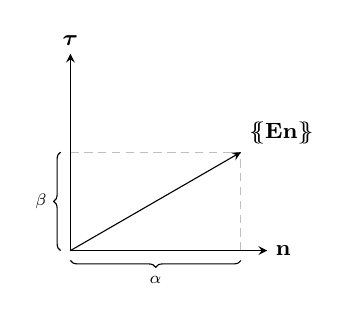
\begin{tikzpicture}[scale=2.5]
	\footnotesize
	\def\theta{30}
	\draw[densely dashed, opacity=.25] ({cos(\theta)},0) -- ({cos(\theta)},{sin(\theta)}); 
	\draw[densely dashed, opacity=.25] (0,{sin(\theta)}) -- ({cos(\theta)},{sin(\theta)}); 
	\draw[->, >=stealth] (0,0) -- (1,0) node[right] {$\mat{n}$}; 
	\draw[->, >=stealth] (0,0) -- ({cos(\theta)}, {sin(\theta)}) node[above right] {$\avg{\mat{E}\mat{n}}$}; 
	\draw[->, >=stealth] (0,0) -- (0,1) node[above] {$\mat{\tau}$}; 
	\draw[decorate,decoration={brace,amplitude=2.5pt}, xshift=-.5mm] (0,0) -- (0,{sin(\theta)}) node[midway,xshift=-2.5mm] {\scalebox{.75}{$\beta$}}; 
	\draw[decorate,decoration={brace,amplitude=2.5pt}, yshift=-.5mm] ({cos(\theta)},0) -- (0,0) node[midway,yshift=-2.5mm] {\scalebox{.75}{$\alpha$}}; 
\end{tikzpicture}
\end{document}